steam
\section{Event Isolation Flagging}
	
	One challange of increasing the readout speed of the detector is prossesing the the data produced.
	Because of this, any pre-computer data processing possible reduces the load and processing time of the computer system.
	One area where the DAQ's FPGA will be used for this purpose is in \underline{E}vent \underline{I}solation \underline{F}lagging (EIF).
	\par
	Particles traversing the VELO have a probability that they will pass thought the boundry of two or more Super Pixels.
	This will cause multiple SPPs for the same particle.
	As such, the reconstruction of the particles path is a more complicated process than a particle path that only interects with one SP.
	\par
	The aim of EIF is to identify the SPPs that completly describe the paticles interaction with the modual and flag then event as isolated.
	These flagged events will allow the computer systems to prioritise these easier to re-construct paths.
	This reduces event pile up the computer network.

	\subsection{Time Sorting Data}

		Frames arriving the DAQ from the GWT are not time ordered.
		When fully implimented, the LLI will have time sorted the data before the EIF.
		However, the provided simulated data of the VELO not time ordered.
		\par
		In order to test any EIF development, it is nessesary to time order the simulation data.
		This was done using a python script that sorted the SPPs into lists accouring to BCID.
		The stript has three main phases:

		\begin{easylist}
			& Read in SPP and rectrieve BCID.
			& Add SPP to correct list according to BCID.
			& Print list of opposite BCID (i.e. input SPP's BCID + 124 acountting for BCID 256 rolling over to 0) to file.
		\end{easylist}

		As not all BCID's are present, measures where put in place to ensure all BCID lists where outputed in time order, preventing list containing two or more bunch cosses. The time order of the data was tested and confirmed as correct.
		\par
		One advantage of this process is that, regardless of the number of isolated events, the data not longer needs to be sorted by the computer network.
		This further reduced the computational load on the computers.

		\subsection{Bubble Sorting}

		The first step in EIF is to sort all the SPP's that correcpont to the same bunch crossing (Hereforth refered to as a \textit{`data trian'}) by there row.
		\par
		Bubble sorting, when implemented in series processing, is a relitivelty slow sorting algorithum.
		At worst case, Bubble sorting requires $n^2$ itterations to complete the sort.
		However, as FPGA's can easily parralell proccess.
		By making $\frac{n}{2}$ comprisons at a simultaniously (even-odd or odd-even), FPGA Bubble Sorting in the worst case senario only requires $n$ itterations. This is made clear in Figure~\ref{fig:sorting}.

		\begin{figure}[ht]
			\centering
			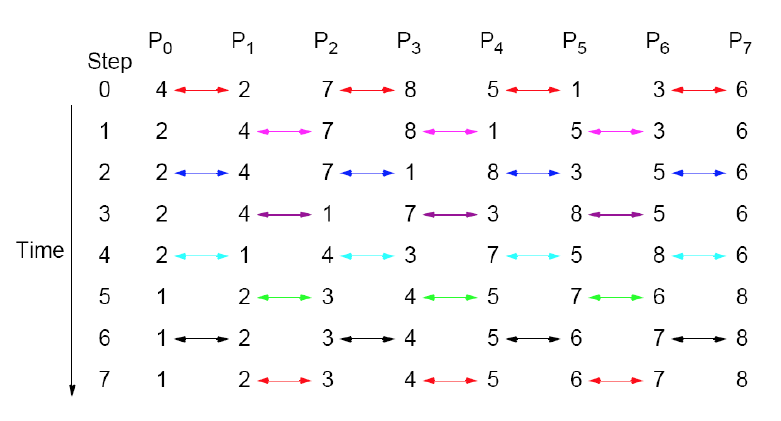
\includegraphics[width=\textwidth]{sorting_diagram}
			\caption{A diagram showing Bubble Sorting in an FPGA.}
			\label{fig:sorting}
		\end{figure}

	\subsection{Isotation Checking}

		Once the data train is sorted by row, each SPP in the train can be compaired against its adjesent SPP's.
		If the SPP is seperated by $>1$ row to both adjesent SPP's, the event is isolated.
		The SPP is then stored as a 31 bit SPP, with the new bit added as the least significant bit (shifting the orrigional SPP 1 bit in significance), with the new bit signaling 1 for isolation and 0 for non-isolated. 

	\subsection{Data Train Overflow} % (fold)
	\label{sub:data_train_overflow}
		
		One limitation of EIF in an FPGA is the limitation on resources. 
		The logic systems are static in design and as such there is a natural need for a cap on the size of datatrain that the EIF system can accept - specifically for the bubble sorting.
		Because of this limitation, the EIF system is required to implement a overflow sytem that will regect data trains above a pre-determined limit, and move them to the next step of the LLI without proccessing them.
		This system is also required to bypass data if a data train arrives at the EIF system before the previous train has been processed - preventing pill up.
		\par
		In order to investigate the limit needed for the overflow, the distribution of data train sizes was investigated. For each ASIC, a graph simular to those in Figure~\ref{fig:asic_datatrain} can be created.

		\begin{figure}[h]
			\centering
			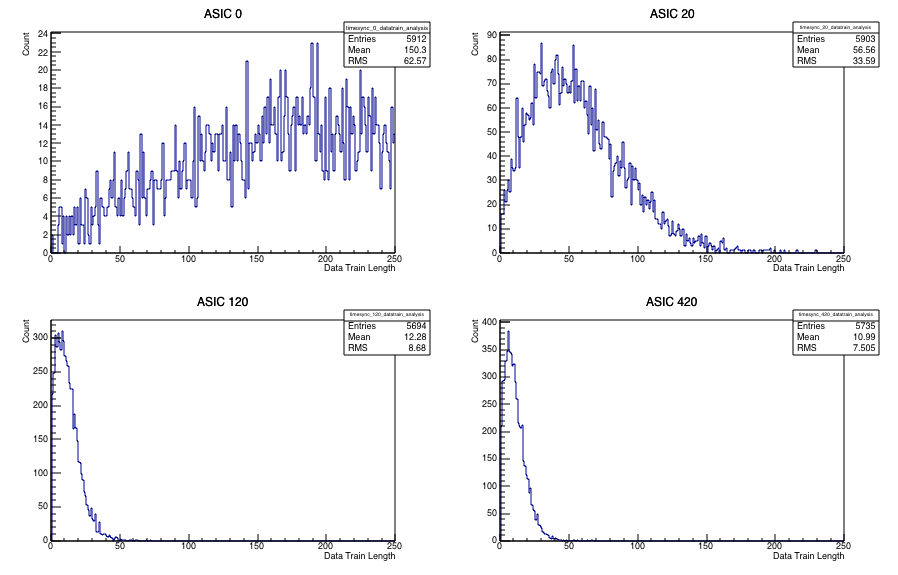
\includegraphics[width=\textwidth]{asic_datatrain_length}
			\caption{The data train length distribution of 4 ASIC chips.}
			\label{fig:asic_datatrain}
		\end{figure}
		\par
		\begin{figure}[h]
			\centering
			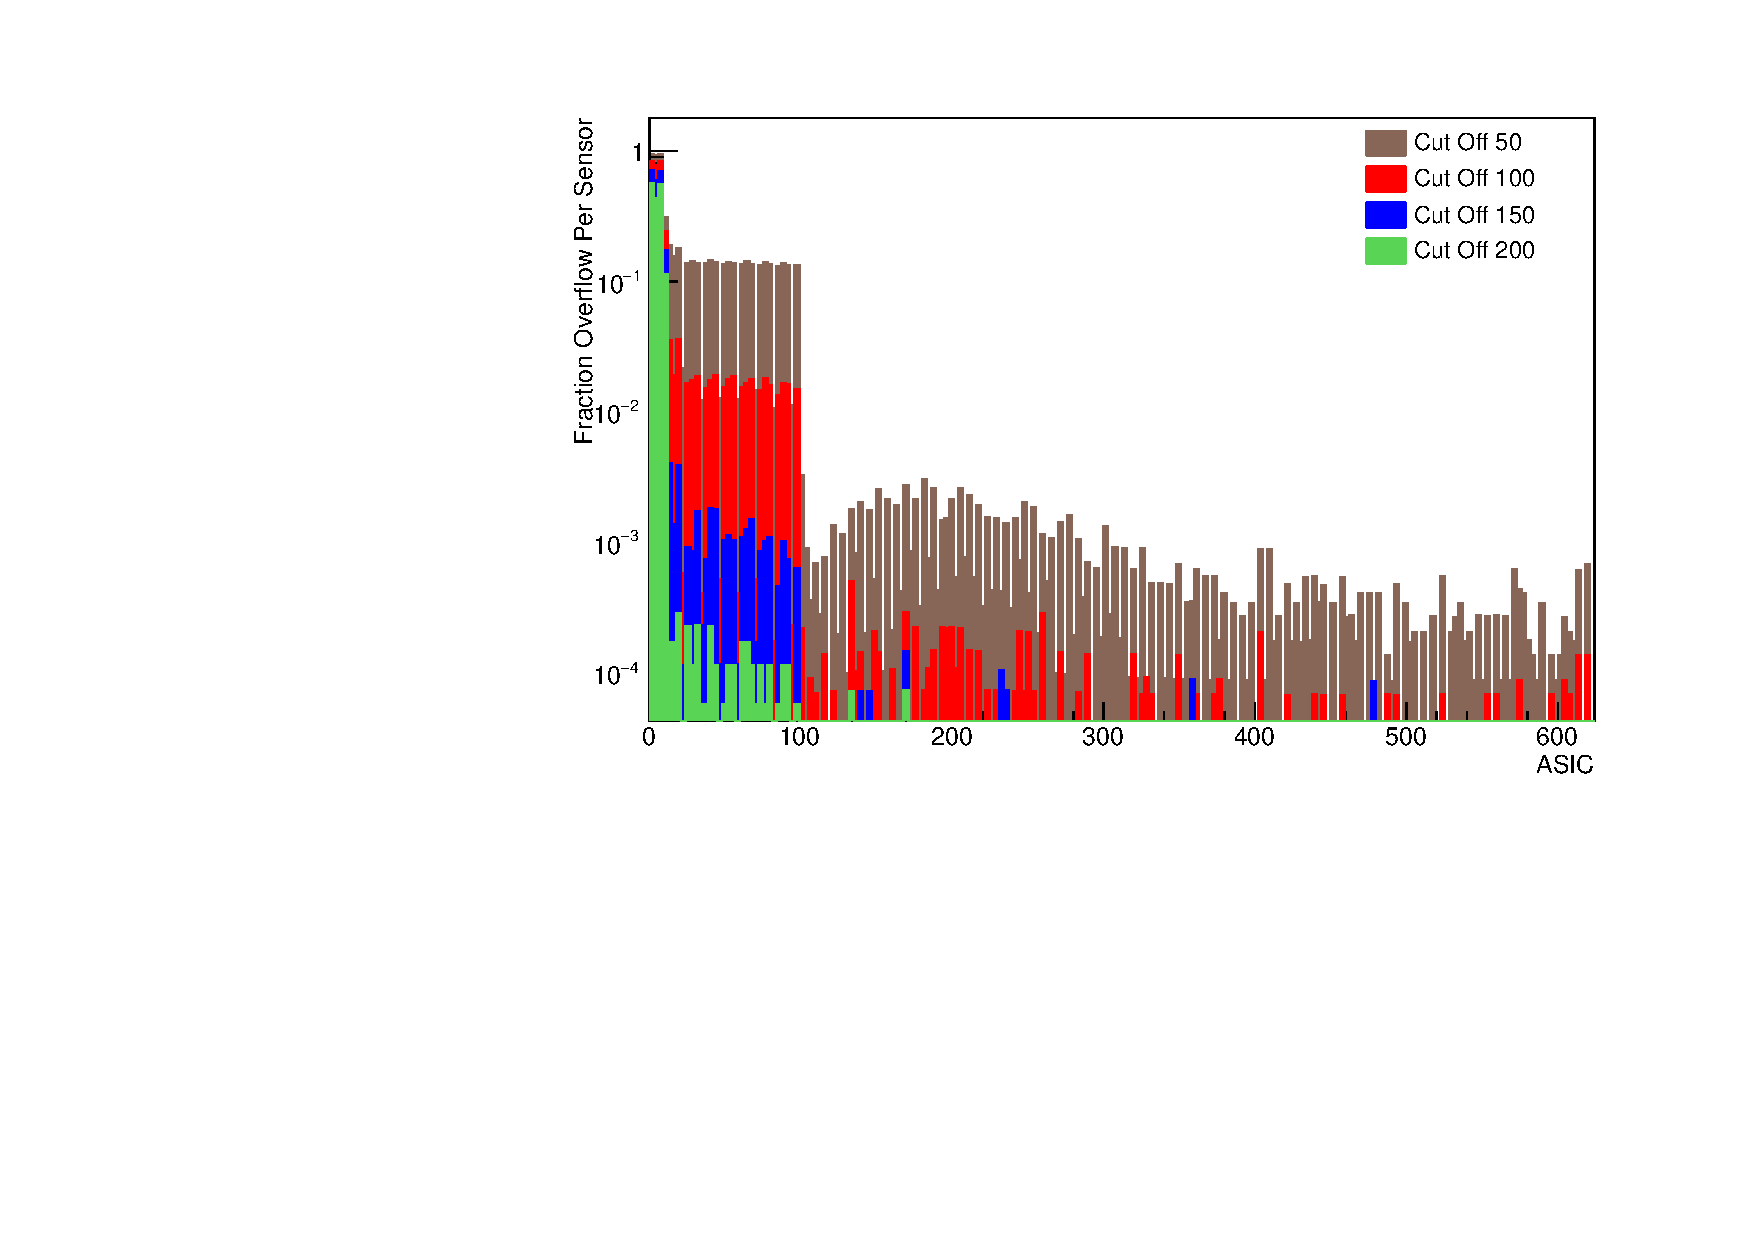
\includegraphics[width=\textwidth]{overflow_graph.pdf}
			\caption{fraction of overflow data trains for four overflow limits.}
			\label{fig:overflow_franction}
		\end{figure}
		More important, however, is the faction of data trains over the bypass limit.
		For four theoretical limits, the fraction of overflow datatrains was calculated from the VELO simulated data, and it shown in Figure~\ref{fig:overflow_franction}.
		This analysis, however, raises questions behond that of the overflow limit.
		The ASIC's below 100 show no simulatity to those above 100.
		\par
		Further investigations as the to structure of the simulated data is shown in Appendix~\ref{app:event_isolation_flagging}.
		From this we learn the large variance in the data (ASIC number > 100) is due to the ASIC's position on the modual this is expected.
		This structure is not consistant across the ACIS's pre and post 100.
		It can be conculed that the simulated data contains a \textit{`bug'} and it now beinging reviewed by the creators of the simulation. No further analysis can be continued on this front until this \textit{`bug'} has been properly investigated.

		% subsection data_train_overflowa (end)

	\subsection{Current Stage of Development} 

		The EIF system is still currently in active VHDL development.
		The current developmently code is still in a stand alone format and not intergrated with the master LLI code.
		Currently created, and ready for stand alone testing, is a bubble sorting module with data in and out systems.
		The module consistance of a top level control entity and a comparison/swap sorting entity.
		The control entity forms a feedback loop passing the ouput of the sorting enity back into its input at each step.
		At each step, the parity of comparison is changed (i.e. odd-even to even-odd).
		\par
		This process continues intill the input and output of the sorting module is identical for two subsequent steps.
		At this point the data is sorted and passed to the output.
		The data flow is more simply demonstraited in Figure~\ref{fig:bubble_data_flow}.

		\begin{figure}[h]
			\centering
			\caption{Data from for the developmental bubble sorting module.}
			\label{fig:bubble_data_flow}
		\end{figure}

		Once testing a bug fixing is complete, the EIF will be expanded to include Isolation Flagging and an overflow as discussed.
		Once the stand alone system is complete, it will be intergrated into the LLI master code and modified to comply with theh LLI data managment systems.